% Template for Cogsci submission with R Markdown

% Stuff changed from original Markdown PLOS Template
\documentclass[10pt, letterpaper]{article}

\usepackage{cogsci}
\usepackage{pslatex}
\usepackage{float}
\usepackage{caption}

% amsmath package, useful for mathematical formulas
\usepackage{amsmath}

% amssymb package, useful for mathematical symbols
\usepackage{amssymb}

% hyperref package, useful for hyperlinks
\usepackage{hyperref}

% graphicx package, useful for including eps and pdf graphics
% include graphics with the command \includegraphics
\usepackage{graphicx}

% Sweave(-like)
\usepackage{fancyvrb}
\DefineVerbatimEnvironment{Sinput}{Verbatim}{fontshape=sl}
\DefineVerbatimEnvironment{Soutput}{Verbatim}{}
\DefineVerbatimEnvironment{Scode}{Verbatim}{fontshape=sl}
\newenvironment{Schunk}{}{}
\DefineVerbatimEnvironment{Code}{Verbatim}{}
\DefineVerbatimEnvironment{CodeInput}{Verbatim}{fontshape=sl}
\DefineVerbatimEnvironment{CodeOutput}{Verbatim}{}
\newenvironment{CodeChunk}{}{}

% cite package, to clean up citations in the main text. Do not remove.
\usepackage{cite}

\usepackage{color}

% Use doublespacing - comment out for single spacing
%\usepackage{setspace}
%\doublespacing


% % Text layout
% \topmargin 0.0cm
% \oddsidemargin 0.5cm
% \evensidemargin 0.5cm
% \textwidth 16cm
% \textheight 21cm

\title{Seeking visual information to support spoken language comprehension}


\author{ {\large \bf Kyle MacDonald}$^1$ (kylem4@stanford.edu), {\large \bf Virginia Marchman}$^1$ (marchman@stanford.edu),  \\ {\large \bf Anne Fernald}$^1$ (afernald@stanford.edu), {\large \bf Michael C. Frank}$^1$ (mcfrank@stanford.edu) 
  \\ $^1$ Department of Psychology Stanford University}

\begin{document}

\maketitle

\begin{abstract}
Efficient language comprehension is a multisensory integration process
where listeners integrate information from the visual and linguistic
signal. But the usefulness of a given information source can vary across
contexts -- as in the case of processing speech in noise or monitoring
another speaker's social cues to reference (e.g., eye gaze). How do
listeners adapt decisions about visual fixation to support
comprehension? Here, we report two experiments that provide evidence for
an adaptive information-seeking account: that listeners alter the
dynamics of gaze during real-time processing to seek additional visual
information when it is useful for supporting comprehension. First, we
show that adults (n=33) and children (n=40, 3-5 y.o.) delayed their eye
movements away from a speaker while processing speech in noise.
Intrestingly, the decision to delay resulted in a speed-accuracy
tradeoff, with more accurate gaze shifts and fewer random responses
(E1). Next, we present results showing one limit of this adaptive
response: both adults (n=33) and children (n=54, 3-5 y.o.) did not delay
eye movements to gather process a post-nominal social cue when the
auditory signal was sufficient to establish reference (E2). Together,
these results suggest that the dynamics of eye movements can flexibly
adapt to the demands of different processing contexts, and that even
very young listeners will seek additional visual information when it is
useful for language comprehension.

\textbf{Keywords:}
eye movements; language processing; information-seeking; speech in
noise; social cue processing
\end{abstract}

\section{Introduction}\label{introduction}

Lanuguage comprehension is fundamentally a multimodal process where
listeners integrate visual and linguistic information to reach a
candidate interpretation. One classic empirical demonstration is the
``McGurk effect'' where a speaker's mouth movement suggests one sound
while their acoustic output suggests another, resulting in the listener
perceiving a third, intermediate sound (J. MacDonald \& McGurk, 1978).
Moreover, theories of speech perception (McClelland, Mirman, \& Holt,
2006) and lexical processing (M. C. MacDonald \& Seidenberg, 2006;
Smith, Monaghan, \& Huettig, 2017) have argued that \emph{interactive}
processes are a defining feature of human language comprehension.

However, the usefulness of different sources of information can vary
depending on features of the listener and features of the surrounding
context. For example, in our prior work, we compared patterns of eye
movements during real-time signed and spoken language comprehension -- a
case where we hypothesized that the value of allocating visual fixations
to the language source being much higher in a visual-manual language. We
found that fluent adults and native ASL learners showed behavioral
signatures of prioritizing information accumuation and accuracy over and
above speed of responding when deciding to look away from a speaker and
to the rest of the visual world (K. MacDonald, Blonder, Marchman,
Fernald, \& Frank, 2017). We proposed an information-maximization
account: that signers' respones were adaptive since responding too
quickly could result in loss of information that would be useful for
sign recognition.

In the work reported here, we aim to test predictions of our
information-maximization account and ask whether features of the
language processing context that modulate the value of visual
information for langauge understanding also change the dynamics of
listeners' \emph{decisions} about visual fixation. We use two
manipulations of context: (1) speech in noise and (2) speech accompanied
with a visual cue to reference (a speaker's eye gaze). We chose the case
of processing speech in noisy environments because we hypothesized that
adding background noise would the auditory signal less reliable, and in
turn make the visual signal more useful. In fact, classic empirical work
on speech perception shows that adults were better able to ``recover''
linguistic information in noisy contexts when they had visual access to
a speaker's face (Erber, 1969). We chose social cue processing because a
speaker who uses a gaze cue provides visual information that completely
disambiguates reference. Moreover, processing social cues are argued to
be a core component of early language acquition and empirical work shows
that gaze following behvaior emerges early in development (Brooks \&
Meltzoff, 2008).

We think these experiments are important for three reasons. First, they
offer a confirmatory test of our explanation for the findings reported
in K. MacDonald et al. (2017), controlling for population-level
differences between signers and spoken language learners. Second, they
inform the generalizability of our account by testing predictions in a
wider variety of contexts, and contexts that are not typically studied
in work on early language processing.

\begin{CodeChunk}
\begin{figure*}[tb]

{\centering 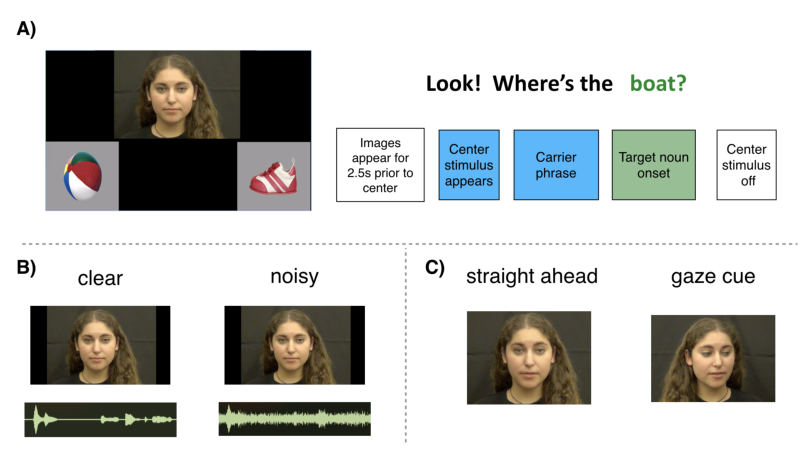
\includegraphics[width=0.7\linewidth]{figs/stimuli-1} 

}

\caption[Stimuli for E1 and E2]{Stimuli for E1 and E2. Panel A shows the layout of the three fixation locations (speaker, target, and distracter), and the timecourse of a single trial. Panel B shows a visual representation of the clear and noisy waveforms used in E1. Panel C shows the social cue manipulation used in E2.}\label{fig:stimuli}
\end{figure*}
\end{CodeChunk}

And third, this work brings together ideas from several rich research
programs and theoretical accounts of language comprehension and vision.
For example, work on language-mediated visual attention shows that
adults and children rapidly shift visual attention upon hearing the name
of an object in the visual scene, with a high proportion of shifts
occurring prior to the offset of the word (Allopenna, Magnuson, \&
Tanenhaus, 1998; Tanenhaus, Spivey-Knowlton, Eberhard, \& Sedivy, 1995).
These findings have led to debates about whether language-mediated
shifts in eye gaze are automatic as opposed to under the control of the
listener. Empirical work on vision during natural tasks shows that
people overwhelmingly prefer to allocate visual fixations towards
\emph{goal-relevant} aspects of the visual world -- e.g., an upcoming
obstacle while walking (Hayhoe \& Ballard, 2005). These accounts make
the prediction that gaze patterns during language comprehension should
adapt to seek higher value visual information to achieve the goal of
rapid language processing. Finally, work on effortful listening shows
that listeners generate compensatory responses (e.g., increases in
attention and working memory) during more ``challenging'' comprehension
contexts such as processing noisy or accented speech (Van Engen \&
Peelle, 2014). These accounts predict that listeners might compensate
for the reduced quality of the auditory signal by allocating more
attentional resources to gathering higher quality visual information.

\section{Experiment 1}\label{experiment-1}

E1 tests whether our information-maximization account of eye movements
would generalize to a novel and ecologically valid language processing
context -- processing speech in noise. We recorded eye movements during
a real-time language comprehension task where children and adults
processed familiar sentences (e.g., ``Where's the ball?'') while looking
at a simplified visual world with 3 fixation targets (see Fig 1). Using
a within-participants design, we manipulated the signal-to-noise ratio
of the auditory information by adding brown noise. We predicted that
processing speech in noise would increase the value of fixating on the
speaker to gather additional inormation before generating a shift to the
named referent even after the target linguistic item began unfolding in
time.

To test this prediction, we compare the Accuracy and Reaction Times
(RTs) of first shifts across the two conditions. We also present two
model-based analyses that link the observable behavior to underlying
psychological constructs. First, we use an exponentially weighted moving
average (EWMA) method (Vandekerckhove \& Tuerlinckx, 2007) to categorize
participants' gaze shifts as language-driven or random. In contrast to
the standard RT/Accuracy analysis, the EMWA allows us to quantify
differences in participants willingness to generate gaze shifts prior to
collecting sufficient information to seek the named referent. Next, we
use drift-diffusion models (DDMs) (Ratcliff \& Childers, 2015) to ask
whether the behavioral differences in Accuracy and RT are driven by a
more cautious responding strategy or by more efficient information
processing -- a critical distinction for our theoretical account.

\subsection{Method}\label{method}

\subsubsection{Participants}\label{participants}

Participants were native, monolingual English-learning children (\(n=\)
39; 22 F, 17 M) and adults (\(n=\) 31; 22 F, 9. All participants had no
reported history of developmental or language delay and normal vision.
14 participants (11 children, 3 adults) were run but not included in the
analysis because either the eye tracker falied to calibrate or the
participant did not complete the task.

\subsubsection{Stimuli}\label{stimuli}

\emph{Linguistic stimuli.} The stimuli were recorded in a sound-proof
room and featured two female speakers who used natural child-directed
speech and said one of two phrases: ``Hey! Can you find the (target
word)''" or ``Look! Where's the (target word) -- see panel A of Fig 1.
The target words were: ball, bunny, boat, bottle, cookie, juice,
chicken, and shoe. The target words varied in length (shortest = 411.68
ms, longest = 779.62 ms) with an average length of 586.71 ms.

\emph{Noise manipulation}. To create the noisy stimuli, we convolved the
recordings with Brown noise using the Audacity audio editor. The average
signal-to-noise ratio\footnote{The ratio of signal power to the noise
  power, with values greater than 0 dB indicating more signal than
  noise.} in the noise condition was 2.87 dB compared to the clear
condition, which was 35.05 dB.

\emph{Visual stimuli.} The image set consisted of colorful digitized
pictures of objects presented in fixed pairs with no phonological
overlap between the target and the distracter image (cookie-bottle,
boat-juice, bunny-chicken, shoe-ball). Side of target picture was
counterbalanced across trials.

\subsubsection{Design and procedure}\label{design-and-procedure}

Participants viewed the task on a screen while their gaze was tracked
using an SMI RED corneal-reflection eye-tracker mounted on an LCD
monitor, sampling at 60 Hz. The eye-tracker was first calibrated for
each participant using a 6-point calibration. On each trial,
participants saw two images of familiar objects on the screen for two
seconds before the center stimulus appeared (see Fig 1). Then they
processed the target sentence -- which consisted of a carrier phrase, a
target noun, and a question -- followed by two seconds without language
to allow for a response. Child participants saw 32 trials (16 noise
trials; 16 clear trials) with several filler trials interspersed to
maintain interest. Adult participants saw 64 trials (32 noise; 32
clear).

\subsection{Results and Discussion}\label{results-and-discussion}

\subsubsection{Analysis plan}\label{analysis-plan}

First, we present behavioral analyses of First Shift Accuracy and
Reaction Time (RT). RT corresponds to the latency to shift away from the
central stimulus to either picture measured from onset of the target
noun in the linguistic stimuli (we log transformed all RTs prior to
analysis). Accuracy corresponds to whether the participant's first gaze
shift landed on the target or the distracter picture. We used the
\texttt{rstanarm} (Gabry \& Goodrich, 2016) package to fit Bayesian
mixed-effects regression models. The mixed-effects approach allowed us
to model the nested structure in our data (multiple trials for each
participant; and a within-participants manipulation) by including random
intercepts for each participant and item, and a random slope for each
item and noise condition. We used Bayesian estimation to quantify the
uncertainty in our point estimates of the group means and condition
differences. To communicate this uncertainty we report the 95\% Highest
Density Interval (HDI), which provides a range of credible values given
the data and model. All analysis code can be found in the online
repository for this project:
\url{https://github.com/kemacdonald/speed-acc/R/analysis}.

Next, we present the two model-based analyses -- the EWMA and HDDM --
discussed in the introduction. Again, the goal of these models is to
move beyond a description of the data and map behavioral differences in
eye movements to underlying psychological variables. First, we use an
EWMA method to model changes in random shifting behavior as a function
of delays in responding (i.e., RT). For each RT, the model generates two
values: a ``control statistic'' (\textbf{CS}, which captures the running
average accuracy of first shifts) and an ``upper control limit''
(\textbf{UCL}, which captures the pre-defined threshold when gaze shifts
would be categorized as deviating from random responding). Here, the CS
is an expectation of random shifting to either the target or the
distracter image (nonlanguage-driven shifts), modeled a Bernoulli
process with \(P(success) = 0.5\). As participants delay their response,
we assume that they have gathered more information and should become
more accurate, which we model a Bernoulli process with
\(P(success) > 0.5\). Using this model, we can quantify and compare: a)
the cutoff point when the CS exceeds the UCL in the RT distribution,
indicating the processing time required before participants generated
language-driven shifts and b) the proportion of all gaze shifts that the
model categorizes as language-driven vs.~nonlanguage-driven.

Finally, we took the shifts that were categorized as language-driven by
the EWMA and fit a hierarchical Bayesian drift-diffusion model (HDDM) to
quantify differences in the underlying decision process that led to
different patterns of behavior. We chose to implement a hierarchical
Bayesian version of the DDM using the HDDM Python package (Wiecki,
Sofer, \& Frank, 2013) since we had relatively few trials from the child
participants and recent simulation studies have shown that the HDDM
approach was better than other DDM fitting methods for small data sets
(Ratcliff \& Childers, 2015). The model assumes that people accumulate
noisy evidence in favor of one alternative with a response generated
when the evidence crosses a pre-defined decision threshold. Here, we
focus on two parameters of interest that map onto meaningful decision
variables that we hypothesized would vary across our conditions:
\textbf{boundary separation}, which indexes the amount of evidence
gathered before generating a response (higher values suggest more
cautious responding) and \textbf{drift rate}, which indexes the amount
of evidence accumulated per unit time (higher values suggest more
efficient processing of the stimulus).

\begin{CodeChunk}
\begin{figure*}[tb]

{\centering 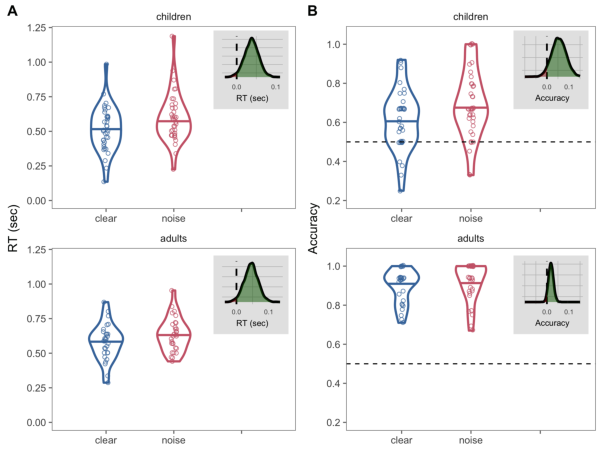
\includegraphics[width=0.9\linewidth]{figs/noise_acc_rt_e1_plot-1} 

}

\caption[Behavioral results from E1]{Behavioral results from E1. Panel A shows violin plots representing the distribution of median RTs for each participant in each condition. The dark red points represent the most likely estimate of the group mean with the error bars showing the 95\% Highest Density Interval. The grey inset plot shows the full posterior distribution of plausible RT differences across conditions with the vertical dashed line representing the null value of zero condition difference. The green shading represents estimates above the null value and the red shading represents estimates below the null value. Panel B shows the same information but for First Shift Accuracy.}\label{fig:noise_acc_rt_e1_plot}
\end{figure*}
\end{CodeChunk}

\subsubsection{Behavioral analyses}\label{behavioral-analyses}

\emph{RT.} To make RTs more suitable for modeling on a linear scale, we
analyzed responses in log space using a logistic transformation, with
the final model was specified as:
\texttt{$log(RT) \sim noise\_condition + age\_group + (sub\_id + noise\_condition \mid item)$}.
Panel A of Figure 2 shows the data distribution for each participant's
RT, the estimates of condition means, and the full posterior
distribution of the estimated difference between the noise and clear
conditions. Both children and adults were slower to identify the target
in the noise condition (Children \(M_{noise}\) = 0.5 ms; Adult
\(M_{noise}\) = 0.6 ms), as compared to the clear condition (Children
\(M_{clear}\) = 0.46 ms; Adult \(M_{clear}\) = 0.55 ms). RTs in the
noise condition were 42.17 ms slower on average, with a 95\% HDI from
1.58 ms to 82.97 ms that did not include the null value of zero
condition difference.

\emph{Accuracy.} Next, we modeled adults' and children's first shift
accuracy using a mixed-effects logistic regression with the same
specifications (see Panel B of Fig 2). Overall, both groups responded at
rates different from a model of random behavior (null value of \(0.5\)
falling well outside the lower bound of all group means). Adults were
more accurate (\(M_{adults} =\) 90\%) compared to children
(\(M_{adults} =\) 62\%). Both groups tended to be more accurate in
shifting to the target image in the noise condition (Children
\(M_{noise}\) = 67\%; Adult \(M_{noise}\) = 92\%) as compared to the
clear condition (Children \(M_{clear}\) = 62\%; Adult \(M_{clear}\) =
90\%). Accuracy in the noise condition was 4\% higher on average, with a
95\% HDI from -1\% to 11\%.Note that while the null value of zero
difference falls within the 95\% HDI, 95\% of the credible values fall
below the null, providing evidence for higher accuracy in the more
challenging noise condition.

\subsubsection{Model-based analyses}\label{model-based-analyses}

\begin{table}[b]
\centering
\begin{tabular}{lllrrr}
  \hline
model & parameter & contrast & MAP & hdi\_lower & hdi\_upper \\ 
  \hline
EWMA & Cut point & age\_group & 0.21 & 0.18 & 0.24 \\ 
  EWMA & Cut point & noise\_condition & 0.04 & 0.01 & 0.06 \\ 
  EWMA & Prop. language-driven & age\_group & -0.47 & -0.49 & -0.44 \\ 
  EWMA & Prop. language-driven & noise\_condition & 0.12 & 0.09 & 0.15 \\ 
   \hline
\end{tabular}
\caption{EWMA and HDDM results for E1.} 
\end{table}

\emph{EWMA.}

\emph{HDDM.}

\section{Experiment 2}\label{experiment-2}

\subsection{Method}\label{method-1}

\subsubsection{Participants}\label{participants-1}

XX Stanford undergraduates participated (XX male, XX females) for course
credit. All participants were monolingual, native English speakers and
had normal vision.

\subsubsection{Stimuli}\label{stimuli-1}

Audio and visual stimuli were identical to the Face and Bullseye tasks
in E1. We included a new center fixation stimulus type: printed text.
The text was displayed in a white font on a black background and was
programmed such that only a single word appeared on the screen, with
each word appearing for the same duration as the corresponding word in
the spoken language stimuli.

\subsubsection{Design and procedure}\label{design-and-procedure-1}

The design was nearly identical to E1, with the exception of a change to
a within-subjects manipulation where each participant completed all four
tasks (Bullseye, Face, Text, and Text-no-audio). In the Text condition,
spoken language accompanied the printed text. In the Text-no-audio
condition, the spoken language stimulus was removed. Participants saw a
total of 128 trials while their eye movements were tracked using
automated eye-tracking software.

\subsection{Results and Discussion}\label{results-and-discussion-1}

\subsubsection{Behavioral analyses}\label{behavioral-analyses-1}

\emph{RT.}

\emph{Accuracy.}

\subsubsection{Model-based analyses}\label{model-based-analyses-1}

\emph{EWMA.}

\emph{HDDM.}

\section{General Discussion}\label{general-discussion}

Language comprehension can be facilitated by fixating on relevant
features of the nonlinguistic visual world or on the speaker. But how do
we decide where to look? We propose that eye movements during language
processing reflect a sensitivity to the tradeoffs of gathering different
kinds of information. We found that young ASL-learners generated slower
but more accurate shifts away from a language source and produced a
smaller proportion of nonlanguage-driven shifts compared to spoken
language learners. We found the same pattern of behavior within a sample
of English-speaking adults processing displays of printed text compared
to spoken language. These results suggest that as the value of fixating
on a location to gather information about the linguistic signal
increases, eye movements to the \emph{rest} of the visual world become
less useful and occur less often.

Our work here attempts to synthesize results from different populations
and stimuli in a single framework, but it has several limitations that
we hope will pave the way for future work. First, we have not performed
a confirmatory test of the DDM findings: both ASL-learners (E1) and
adults processing language from a person (E2) prioritize accuracy over
speed. So these findings, while interesting, are preliminary. Second, we
do not know what might be driving the population differences in E1. It
could be that ASL-learners' massive experience dealing with competition
for visual attention leads to changes in the deployment of eye movements
during language comprehension. Or, it could be that the in-the-moment
constraints of processing a visual language cause different fixation
behaviors. Finally, we used a very simple visual world, with only three
places to look, and very simple linguistic stimuli, especially for the
adults in E2. Thus it remains an open question how these results might
scale up to more complex language information and visual environments.

This work attempts to integrate top-down, goal-based models of vision
(Hayhoe \& Ballard, 2005) with work on language-driven eye movements
(Allopenna et al., 1998). While we chose to start with two case studies
-- ASL and text processing -- we think the account is more general and
that there are many real world situations where people must negotiate
the tradeoff between gathering more information about language or about
the world: e.g., processing spoken language in noisy environments or at
a distance; or early in language learning when children are acquiring
new words and often rely on nonlinguistic cues to reference such as
pointing or eye gaze. Overall, we hope this work contributes to a
broader account of eye movements during language comprehension that can
explain fixation behaviors across a wider variety of populations,
processing contexts, and during different stages of language learning.

\section{Acknowledgements}\label{acknowledgements}

We are grateful to the families who participated in this research.
Thanks to Tami Alade and Hannah Slater for help with data collection.
This work was supported by an NSF GRFP to KM.

\section{References}\label{references}

\setlength{\parindent}{-0.1in} \setlength{\leftskip}{0.125in} \noindent

\hypertarget{refs}{}
\hypertarget{ref-allopenna1998tracking}{}
Allopenna, P. D., Magnuson, J. S., \& Tanenhaus, M. K. (1998). Tracking
the time course of spoken word recognition using eye movements: Evidence
for continuous mapping models. \emph{Journal of Memory and Language},
\emph{38}(4), 419--439.

\hypertarget{ref-brooks2008infant}{}
Brooks, R., \& Meltzoff, A. N. (2008). Infant gaze following and
pointing predict accelerated vocabulary growth through two years of age:
A longitudinal, growth curve modeling study. \emph{Journal of Child
Language}, \emph{35}(01), 207--220.

\hypertarget{ref-erber1969interaction}{}
Erber, N. P. (1969). Interaction of audition and vision in the
recognition of oral speech stimuli. \emph{Journal of Speech and Hearing
Research}, \emph{12}(2), 423--425.

\hypertarget{ref-gabry2016rstanarm}{}
Gabry, J., \& Goodrich, B. (2016). Rstanarm: Bayesian applied regression
modeling via stan. r package version 2.10. 0.

\hypertarget{ref-hayhoe2005eye}{}
Hayhoe, M., \& Ballard, D. (2005). Eye movements in natural behavior.
\emph{Trends in Cognitive Sciences}, \emph{9}(4), 188--194.

\hypertarget{ref-macdonald1978visual}{}
MacDonald, J., \& McGurk, H. (1978). Visual influences on speech
perception processes. \emph{Attention, Perception, \& Psychophysics},
\emph{24}(3), 253--257.

\hypertarget{ref-macdonald2017info}{}
MacDonald, K., Blonder, A., Marchman, V. and, Fernald, A., \& Frank, M.
C. (2017). An information-seeking account of eye movements during spoken
and signed language comprehension. In \emph{Proceedings of the 39th
annual conference of the cognitive science society}.

\hypertarget{ref-macdonald2006constraint}{}
MacDonald, M. C., \& Seidenberg, M. S. (2006). Constraint satisfaction
accounts of lexical and sentence comprehension. \emph{Handbook of
Psycholinguistics}, \emph{2}, 581--611.

\hypertarget{ref-mcclelland2006there}{}
McClelland, J. L., Mirman, D., \& Holt, L. L. (2006). Are there
interactive processes in speech perception? \emph{Trends in Cognitive
Sciences}, \emph{10}(8), 363--369.

\hypertarget{ref-ratcliff2015individual}{}
Ratcliff, R., \& Childers, R. (2015). Individual differences and fitting
methods for the two-choice diffusion model of decision making.
\emph{Decision}, \emph{2}(4), 237--279.

\hypertarget{ref-smith2017multimodal}{}
Smith, A. C., Monaghan, P., \& Huettig, F. (2017). The multimodal nature
of spoken word processing in the visual world: Testing the predictions
of alternative models of multimodal integration. \emph{Journal of Memory
and Language}, \emph{93}, 276--303.

\hypertarget{ref-tanenhaus1995integration}{}
Tanenhaus, M. K., Spivey-Knowlton, M. J., Eberhard, K. M., \& Sedivy, J.
C. (1995). Integration of visual and linguistic information in spoken
language comprehension. \emph{Science}, \emph{268}(5217), 1632.

\hypertarget{ref-van2014listening}{}
Van Engen, K. J., \& Peelle, J. E. (2014). Listening effort and accented
speech. \emph{Frontiers in Human Neuroscience}, \emph{8}.

\hypertarget{ref-vandekerckhove2007fitting}{}
Vandekerckhove, J., \& Tuerlinckx, F. (2007). Fitting the ratcliff
diffusion model to experimental data. \emph{Psychonomic Bulletin \&
Review}, \emph{14}(6), 1011--1026.

\hypertarget{ref-wiecki2013hddm}{}
Wiecki, T. V., Sofer, I., \& Frank, M. J. (2013). HDDM: Hierarchical
bayesian estimation of the drift-diffusion model in python.
\emph{Frontiers in Neuroinformatics}, \emph{7}, 14.

\end{document}
